\textbf{Актуальность исследования:}

Компьютеризация и информатизация различных сфер общества и производства неизменно
сопровождается созданием специфических программных и аппаратных средств.

\begin{figure}[!htbp]
    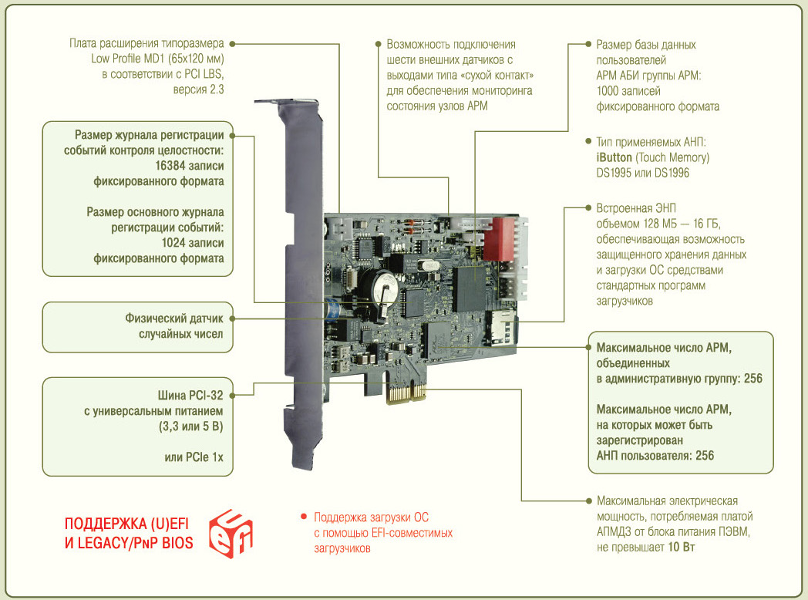
\includegraphics[width=\textwidth,height=\textheight,keepaspectratio]{images/apmdz.png}
    \caption{Пример специфического аппаратного обеспечения: АПМДЗ Максим-М1\label{fig:apmdz}}
\end{figure}

Разработка аппаратного обеспечения практически никогда не обходится без создания
прикладного програмного обеспечения.
Правильное проектирование архитектуры ПО и выделение уровней абстракции позволяет
разрабатывать программное обеспечение и аппаратное обеспечение параллельно, но
до определенного уровня.

В теории теория и практика не различаются, но не на практике.
Для тестирования и отладки прикладного ПО в конечном счете понадобится аппаратное обеспечение,
но зачастую им сложно обеспечить всю команду разработчиков, особенно на ранних стадиях.
Причиной этому могут быть экономические, логистические, производственные или временные проблемы.

Но даже если обеспечить всех разработчиков необходимыми стендами, то при проявлении
проблем во взаимодействии ПО и АО, аппаратное обеспечение придется отправлять на доработку,
после чего снова печатать, доставлять и собирать стенды, что неизбежно приводит к экономическим
и временным издержкам, которые, в свою очередь, повышают затраты на завершение проекта в срок.

Исправить и запустить ПО на поздних этапах проектирования легче, чем исправить и перевыпустить схему.

\textbf{Проблемная ситуация в области объекта исследований:}

Отсутствие быстрого способа создания эмуляторов специализированного аппаратного обеспечения, что отражается
экономических аспектах конечного продукта.

\textbf{Причины сложившейся ситуации:}
\begin{enumerate}[label={\arabic*)}]
    \item отсутствие формализованного подхода к созданию эмуляторов аппаратного обеспечения;
    \item отсутствие универсального метода написания эмуляторов аппаратного обеспечения;
\end{enumerate}

\textbf{Объект исследования:}

Существующие методики поиска НДВ в программном обеспечении.

\textbf{Предмет исследования:}

Программное обеспечение.

\textbf{Цель исследования:}
уменьшение количества ложноположительных и ложноотрицательных срабатываний поиска НДВ.

\textbf{Задачи исследования:}
\begin{enumerate}[label={\arabic*)}]
    \item анализ возможностей нарушителя;
    \item анализ критичности и применимости воздействия нарушителя на ПО;
    \item создание методики выбора инструментов для проверки воздействия нарушителя на ПО;
    \item разработка алгоритма поиска НДВ;
\end{enumerate}
